\documentclass[aspectratio=169]{beamer}
\usepackage[utf8]{inputenc}
\usepackage[english,russian]{babel}
\usepackage{cancel}
\usepackage{amssymb}
\usepackage{stmaryrd}
\usepackage{cmll}
\usepackage{graphicx}
\usepackage{amsthm}
\usepackage{amsmath}
\usepackage{tikz}
\usepackage{multicol}
\usetikzlibrary{patterns,calc}
\usepackage{chronosys}
\usepackage{proof}
\usepackage{multirow}
\usepackage{marvosym}
\usepackage{hyperref}
%\usepackage{tabularx}
\usepackage{comment}
\setbeamertemplate{navigation symbols}{}
%\usetheme{Warsaw}

\newtheorem{thm}{Теорема}[section]
\newtheorem{dfn}{Определение}[section]
\newtheorem{lmm}{Лемма}[section]
\newtheorem{exm}{Пример}[section]
\newtheorem{snote}{Пояснение}[section]

\newcommand{\divisible}%
{\mathrel{\lower.2ex%
\vbox{\baselineskip=0.7ex\lineskiplimit=0pt%
\kern6pt \hbox{.}\hbox{.}\hbox{.}}%
}}

\begin{document}

\newcommand\doubleplus{+\kern-1.3ex+\kern0.8ex}
\newcommand\mdoubleplus{\ensuremath{\mathbin{+\mkern-10mu+}}}


\begin{frame}{}
\LARGE\begin{center}Мощность множеств\end{center}
\end{frame}

\begin{frame}{Отношения}
\begin{dfn}$A \times B := \{\langle a,b \rangle\ |\ a \in A, b \in B\}$

Бинарное отношение --- $R \subseteq A \times B$

Функциональное бинарное отношение (функция) $R$ --- такое, что $\forall x.x\in A\rightarrow\exists !y.\langle x,y\rangle \in R$

$R$ --- инъективная функция, если $\forall x.\forall y.\langle x,t\rangle \in R\with \langle y,t\rangle \in R \rightarrow x=y$.

$R$ --- сюръективная функция, если $\forall y.y \in B\rightarrow\exists x.\langle x,y\rangle\in R$.\end{dfn}
\end{frame}

\begin{frame}{Равномощные множества}
\begin{dfn}Множество $A$ \emph{равномощно} $B$ $(|A|=|B|)$, если существует биекция
$f: A \rightarrow B$.

Множество $A$ имеет мощность, не превышающую мощности $B$ $(|A|\le|B|)$, если существует инъекция $f: A \rightarrow B$.
\end{dfn}
\end{frame}

\begin{frame}{Теорема Кантора-Бернштейна}
\begin{thm}Если $|A| \le |B|$ и $|B| \le |A|$, то $|A| = |B|$.\end{thm}
Заметим, $f: A \rightarrow B$, $g: B \rightarrow A$ --- инъекции, но не обязательно $g(f(x)) = x$.
\begin{proof}
%Пусть $f: A \rightarrow B$ и $g: B \rightarrow A$. Построим биекцию в явном виде. %\begin{enumerate}

Избавимся от множества $B$: пусть $A_0 = A$; $A_1 = g(B)$; $A_{k+2} = g(f(A_k))$.

\vspace{-0.2cm}
\begin{center}\tikz{
\node[inner sep=0, outer sep=0] (A0) at (0,0) {};
\node[inner sep=0, outer sep=0] (A1) at (2,0) {};
\node[inner sep=0, outer sep=0] (A2) at (3,0) {};
\node[inner sep=0, outer sep=0] (A3) at (3.5,0) {};
\node[inner sep=0, outer sep=0] (A4) at (3.75,0) {};
\node[inner sep=0, outer sep=0] (AN) at (4,0) {};
\node[inner sep=0, outer sep=0] (AE) at (6,0) {};

\node (B0) at (0,-1.5) {};
\node (B1) at (2,-1.5) {};
\node (B2) at (3,-1.5) {};
\node (B3) at (3.5,-1.5) {};
\node (B4) at (3.75,-1.5) {};
\node (BN) at (4,-1.5) {};
\node (BE) at (6,-1.5) {};

\fill[gray!80] ($(A0)+(0,0.1)$) rectangle node[pos=0.1,above]{\color{gray} $A_0$} ($(AE)+(0,0.15)$);
\fill[gray!30] ($(A1)+(0,0.2)$) rectangle node[pos=0.1,above]{\color{gray} $A_1$} ($(AE)+(0,0.25)$);
\fill[gray!80] ($(A2)+(0,0.3)$) rectangle node[pos=0.1,above]{\color{gray} $A_2$} ($(AE)+(0,0.35)$);
\fill[gray!30] ($(A3)+(0,0.4)$) rectangle node[pos=0.1,above]{\color{gray} $A_3$} ($(AE)+(0,0.45)$);
\fill[gray!80] ($(AN)+(0,0.5)$) rectangle node[midway,above]{\color{gray} $\cap A_k$} ($(AE)+(0,0.55)$);
%\draw (A3) -- node[midway,above]{$\dots$} (AN) (AE);
%\draw (B0) to (BE);

%\draw (AN) to (BN);

\fill[gray!80] ($(B0)-(0,0.1)$) rectangle node[pos=0.1,below]{\color{gray} $B_0$} ($(BE)-(0,0.15)$);
\fill[gray!80] ($(B1)-(0,0.1)$) rectangle node[pos=0.1,below]{\color{gray} $B_1$} ($(BE)-(0,0.15)$);
\fill[gray!80] ($(B2)-(0,0.1)$) rectangle node[pos=0.1,below]{\color{gray} $B_2$} ($(BE)-(0,0.15)$);
\fill[gray!80] ($(B3)-(0,0.1)$) rectangle node[pos=0.1,below]{\color{gray} $B_3$} ($(BE)-(0,0.15)$);
\fill[gray!80] ($(BN)-(0,0.1)$) rectangle node[midway,below]{\color{gray} $\cap B_k$} ($(BE)-(0,0.15)$);

\fill[gray!30] (4,0) -- (6,0) -- (6,-1.5) -- (4,-1.5);

\fill[gray!30] (3,-1.5) -- (3.5,-1.5) -- (3.75,0) -- (3.5,0);
\fill[gray!30] (0,-1.5) -- (2,-1.5) -- (3,0) -- (2,0);
\fill[gray!30] (3.75,-1.5) -- (3.875,-1.5) -- (3.875+0.0625,0) -- (3.875,0);
\fill[gray!80] (0,0) -- (2,-1.5) -- (3,-1.5) -- (2,0);
\fill[gray!80] (3,0) -- (3.5,-1.5) -- (3.75,-1.5) -- (3.5,0);
\fill[gray!80] (3.75,0) -- (3.875,-1.5) -- (3.875+0.0625,-1.5) -- (3.875,0);
%\draw[dashed,->] (B3) -- (A4);

}\end{center}

\vspace{-0.4cm}

Тогда, если существует $h: A_0 \rightarrow A_1$ --- биекция, то тогда $g^{-1}\circ h: A \rightarrow B$ --- 
требуемая биекция.

%\item Построим биекцию $h: A_0 \rightarrow A_1$\end{enumerate}
\end{proof}

\end{frame}

\begin{frame}{Построение биекции $h: A_0 \rightarrow A_1$}
Пусть $C_k = A_k \setminus A_{k+1}$. Тогда $g(f(C_k)) = g(f(A_k))\setminus g(f(A_{k+1})) = A_{k+2}\setminus A_{k+3} = C_{k+2}$.

\begin{center}\tikz{
\node[inner sep=0, outer sep=0] (A0) at (0,0) {};
\node[inner sep=0, outer sep=0] (A1) at (2,0) {};
\node[inner sep=0, outer sep=0] (A2) at (3,0) {};
\node[inner sep=0, outer sep=0] (A3) at (3.5,0) {};
\node[inner sep=0, outer sep=0] (A4) at (3.75,0) {};
\node[inner sep=0, outer sep=0] (AN) at (4,0) {};
\node[inner sep=0, outer sep=0] (AE) at (6,0) {};

\node (B0) at (0,-1.5) {};
\node (B1) at (2,-1.5) {};
\node (B2) at (3,-1.5) {};
\node (B3) at (3.5,-1.5) {};
\node (B4) at (3.75,-1.5) {};
\node (BN) at (4,-1.5) {};
\node (BE) at (6,-1.5) {};

\fill[gray!80] ($(A0)+(0,0.1)$) rectangle node[pos=0.1,above]{\color{gray} $C_0$} ($(AE)+(0,0.15)$);
\fill[gray!30] ($(A1)+(0,0.1)$) rectangle node[pos=0.1,above]{\color{gray} $C_1$} ($(AE)+(0,0.15)$);
\fill[gray!80] ($(A2)+(0,0.1)$) rectangle node[pos=0.1,above]{\color{gray} $C_2$} ($(AE)+(0,0.15)$);
\fill[gray!30] ($(A3)+(0,0.1)$) rectangle node[pos=0.1,above]{\color{gray} $C_3$} ($(AE)+(0,0.15)$);
\fill[gray!80] ($(AN)+(0,0.1)$) rectangle node[midway,above]{\color{gray} $\cap A_k$} ($(AE)+(0,0.15)$);
\fill[white] ($(A4)+(0,0.1)$) rectangle ($(AN)+(0,0.15)$);
%\draw (A3) -- node[midway,above]{$\dots$} (AN) (AE);
%\draw (B0) to (BE);

%\draw (AN) to (BN);

%\fill[gray!80] ($(B0)-(0,0.1)$) rectangle node[pos=0.1,below]{\color{gray} $B_0$} ($(BE)-(0,0.15)$);
%\fill[gray!80] ($(B1)-(0,0.1)$) rectangle node[pos=0.1,below]{\color{gray} $B_1$} ($(BE)-(0,0.15)$);
%\fill[gray!80] ($(B2)-(0,0.1)$) rectangle node[pos=0.1,below]{\color{gray} $B_2$} ($(BE)-(0,0.15)$);
%\fill[gray!80] ($(B3)-(0,0.1)$) rectangle node[pos=0.1,below]{\color{gray} $B_3$} ($(BE)-(0,0.15)$);
%\fill[gray!80] ($(BN)-(0,0.1)$) rectangle node[midway,below]{\color{gray} $\cap B_k$} ($(BE)-(0,0.15)$);

\fill[gray!30] (4,0) -- (6,0) -- (6,-1.5) -- (4,-1.5);

\fill[gray!30] (3,-1.5) -- (3.5,-1.5) -- (3.75,0) -- (3.5,0);
\fill[gray!30] (0,-1.5) -- (2,-1.5) -- (3,0) -- (2,0);
\fill[gray!30] (3.75,-1.5) -- (3.875,-1.5) -- (3.875+0.0625,0) -- (3.875,0);
\fill[gray!80] (0,0) -- (2,-1.5) -- (3,-1.5) -- (2,0);
\fill[gray!80] (3,0) -- (3.5,-1.5) -- (3.75,-1.5) -- (3.5,0);
\fill[gray!80] (3.75,0) -- (3.875,-1.5) -- (3.875+0.0625,-1.5) -- (3.875,0);
%\draw[dashed,->] (B3) -- (A4);

}\end{center}

Тогда определим $h(x)$ следующим образом:

\tikz{
\node (F) at (-3,-1) {$h(x) = \left\{\begin{array}{ll} x, & x \in C_{2k+1} \vee x \in \cap A_k\\
                g(f(x)), & x \in C_{2k}\end{array}\right.$};


\node[inner sep=0, outer sep=0] (A0) at (0,0) {};
\node[inner sep=0, outer sep=0] (A1) at (2,0) {};
\node[inner sep=0, outer sep=0] (A2) at (3,0) {};
\node[inner sep=0, outer sep=0] (A3) at (3.5,0) {};
\node[inner sep=0, outer sep=0] (A4) at (3.75,0) {};
\node[inner sep=0, outer sep=0] (AN) at (4,0) {};
\node[inner sep=0, outer sep=0] (AE) at (6,0) {};

\node (B0) at (0,-1.5) {};
\node (B1) at (2,-1.5) {};
\node (B2) at (3,-1.5) {};
\node (B3) at (3.5,-1.5) {};
\node (B4) at (3.75,-1.5) {};
\node (BN) at (4,-1.5) {};
\node (BE) at (6,-1.5) {};

\fill[gray!80] ($(A0)+(0,0.1)$) rectangle node[pos=0.1,above]{\color{gray} $C_0$} ($(AE)+(0,0.15)$);
\fill[gray!30] ($(A1)+(0,0.1)$) rectangle node[pos=0.1,above]{\color{gray} $C_1$} ($(AE)+(0,0.15)$);
\fill[gray!80] ($(A2)+(0,0.1)$) rectangle node[pos=0.08,above]{\color{gray} $C_2$} ($(AE)+(0,0.15)$);
\fill[gray!30] ($(A3)+(0,0.1)$) rectangle node[pos=0.08,above]{\color{gray} $C_3$} ($(AE)+(0,0.15)$);
\fill[gray!80] ($(AN)+(0,0.1)$) rectangle node[midway,above]{\color{gray} $\cap A_k$} ($(AE)+(0,0.15)$);
\fill[white] ($(A4)+(0,0.1)$) rectangle ($(AN)+(0,0.15)$);
%\draw (A3) -- node[midway,above]{$\dots$} (AN) (AE);
%\draw (B0) to (BE);

%\draw (AN) to (BN);

%\fill[gray!80] ($(B0)-(0,0.1)$) rectangle node[pos=0.1,below]{\color{gray} $C_0$} ($(BE)-(0,0.15)$);
\fill[gray!30] ($(B1)-(0,0.1)$) rectangle node[pos=0.1,below]{\color{gray} $C_1$} ($(BE)-(0,0.15)$);
\fill[gray!80] ($(B2)-(0,0.1)$) rectangle node[pos=0.08,below]{\color{gray} $C_2$} ($(BE)-(0,0.15)$);
\fill[gray!30] ($(B3)-(0,0.1)$) rectangle node[pos=0.08,below]{\color{gray} $C_3$} ($(BE)-(0,0.15)$);
\fill[gray!80] ($(BN)-(0,0.1)$) rectangle node[midway,below]{\color{gray} $\cap A_k$} ($(BE)-(0,0.15)$);
\fill[white] ($(B4)-(0,0.1)$) rectangle ($(BN)-(0,0.15)$);

\fill[gray!30] (4,0) -- (6,0) -- (6,-1.5) -- (4,-1.5);
\fill[gray!30] (2,-1.5) -- (3,-1.5) -- (3,0) -- (2,0);
%\fill[gray!30] (0,-1.5) -- (2,-1.5) -- (3.5,0) -- (3,0);
\fill[gray!30] (3.5,-1.5) -- (3.75,-1.5) -- (3.75,0) -- (3.5,0);
\fill[gray!80] (0,0) -- (3,-1.5) -- (3.5,-1.5) -- (2,0);
\fill[gray!80] (3,0) -- (3.75,-1.5) -- (3.875,-1.5) -- (3.5,0);
%\fill[gray!80] (3.75,0) -- (3.875,-1.5) -- (3.875+0.0625,-1.5) -- (3.875,0);
%\draw[dashed,->] (B3) -- (A4);

}

\end{frame}

\begin{frame}{Кардинальные числа}
\begin{dfn}Кардинальное число --- наименьший ординал, не равномощный никакому меньшему:
$$\forall x.x \in c \rightarrow |x| < |c|$$\end{dfn}
\begin{thm}Конечные ординалы --- кардинальные числа.\end{thm}
\begin{dfn}Мощность множества $(|S|)$ --- равномощное ему кардинальное число.\end{dfn}
\end{frame}

\begin{frame}{Диагональный метод}
\begin{lmm}$|\mathbb{R}| > |\mathbb{N}|$\end{lmm}
\begin{proof}Рассмотрим $a \in (0,1)$ и десятичную запись: $0.a_0a_1a_2\dots$.
Пусть существует биективная $f: \mathbb{N}\rightarrow (0,1)$.
По функции найдём значение $\sigma$, не являющееся образом никакого натурального числа.

\begin{center}\begin{tabular}{cc|ccccccl}
 $n$ &  $f(n)$ & $f(n)_0$ & $f(n)_1$ & $f(n)_2$ & $f(n)_3$ & $f(n)_4$ & $f(n)_5$ & $\dots$ \\\hline
 $n_0$ &  0.3  &  \color{red}3    & 0    &  0  &  0  &  0  &  0 & $\dots$ \\
 $n_1$ & $\pi/10$ &  3  & \color{red}1    &  4  &  1  &  5  &  9 & $\dots$ \\
 $n_2$ & $1/7$   & 1 &   4    &  \color{red}2  &  8  &  5  &  7 & $\dots$ \\\hline\pause
       & $\sigma$ & 8 &  6 &        7 &   \multicolumn{4}{l}{$\dots \sigma_k = (f(n_k)_k+5) \% 10$}
\end{tabular}\end{center}

%Заметим, что при любом $n \in \mathbb{N}$ выполнено $|\sigma_n - f(n)_n| = 5$.
\end{proof}
\end{frame}

\begin{frame}{Теорема Кантора}
\begin{thm}$|\mathcal{P}(S)| > |S|$\end{thm}
\begin{proof}Пусть $S = \{a,b,c,\dots\}$

\begin{center}\begin{tabular}{c|cccl}
$n$ & $a \in f(n)$ & $b \in f(n)$ & $c \in f(n)$ & $\dots$ \\\hline
$a$ & \color{red}И & Л & И \\
$b$ &       Л & \color{red}Л& И \\
$c$ &   И & И & \color{red}И\\\hline
   & Л & И & Л & $y \notin f(y)$
\end{tabular}\end{center}\pause

Пусть $f: S \rightarrow \mathcal{P}(S)$ --- биекция. Тогда 
$\sigma = \{ y\in S\ |\ y\notin f(y)\}$. Пусть $f(x) = \sigma$.
Но $x \in f(x)$ тогда и только тогда, когда $x \notin \sigma$, то есть $f(x) \ne \sigma$.
\end{proof}
\end{frame}

\begin{frame}[fragile]{О буквах}
\begin{comment}
\begin{tabular}{c|lm{4cm}|c|l}
иероглиф & финикийский & евр. &  лат./греч./кир.\\\hline
\begin{minipage}{2cm}\center\footnotesize
\includegraphics[scale=0.25]{pics/lection-14-ox}\\голова быка\end{minipage}&
  \begin{minipage}{2cm}\center\footnotesize%
    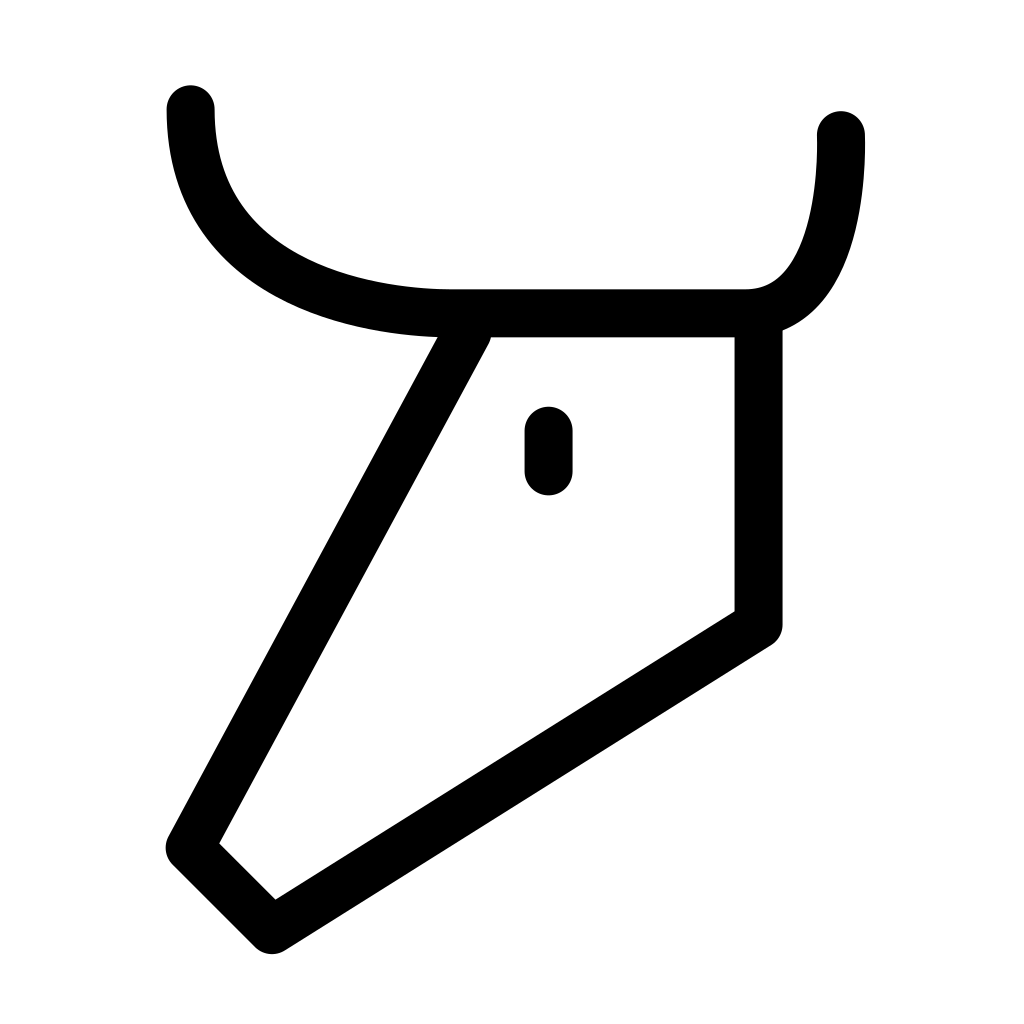
\includegraphics[scale=0.01]{pics/lection-14-ph-aleph-proto}
    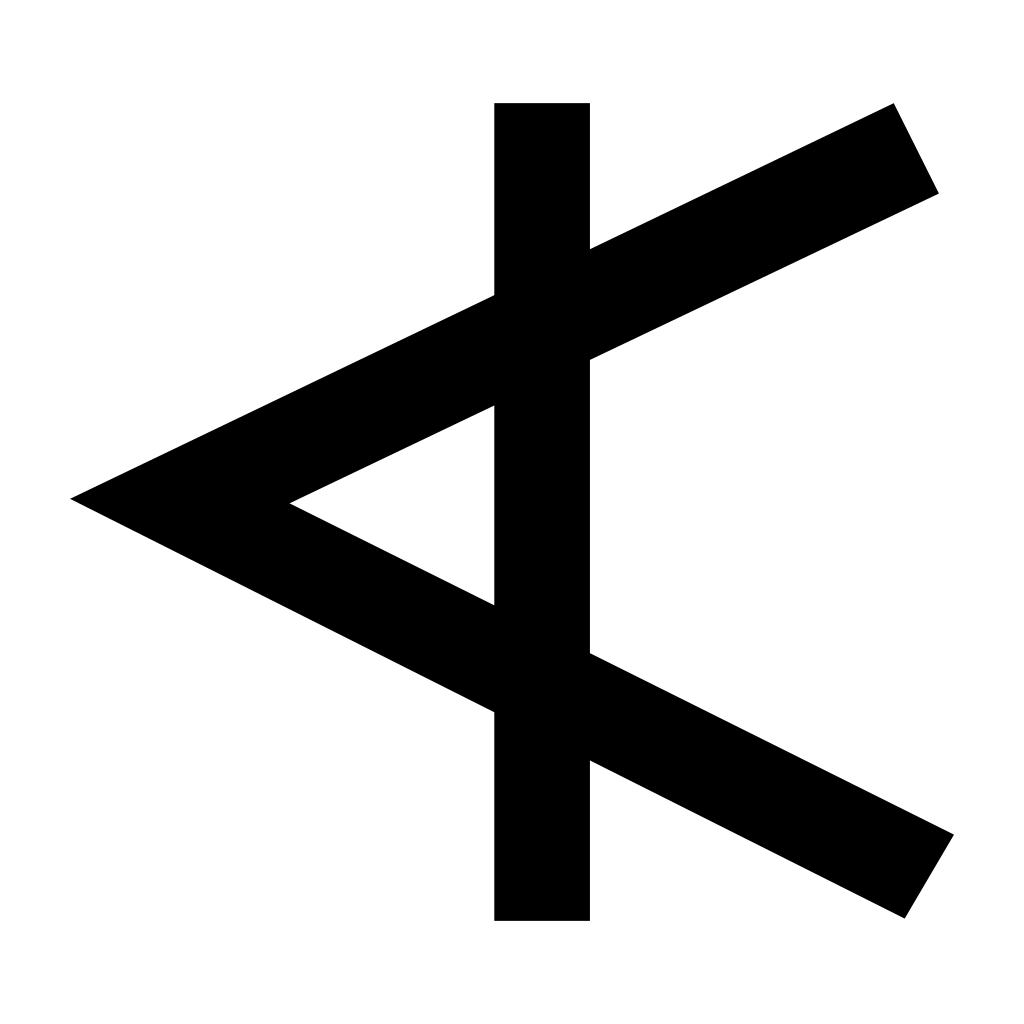
\includegraphics[scale=0.01]{pics/lection-14-ph-aleph}\\'алф\end{minipage} &  $\aleph$ алеф &  a, $\alpha$\\
\begin{minipage}{2cm}\center\footnotesize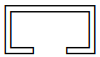
\includegraphics[scale=0.25]{pics/lection-14-house}\\дом\end{minipage} & &  $\beth$ бейт &  b, Б, $\beta$\\
\begin{minipage}{2cm}\center\footnotesize
\includegraphics[scale=0.25]{pics/lection-14-throwstick}\\метательная палка\end{minipage} & гамл &   $\gimel$ гимель &  Г\\
\begin{minipage}{2cm}\center\footnotesize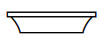
\includegraphics[scale=0.25]{pics/lection-14-door}\\дверь/рыба\end{minipage} & далт & далет &  Д, D, $\Delta$
\end{tabular}
\end{comment}

\footnotesize
\begin{center}
\begin{tabular}{c|c|c|c}
 иероглиф &  протосинайский/финик. &  греч./лат./кир. &  евр.\\\hline
&&&\\

\includegraphics[scale=0.25]{pics/lection-14-ox} &
    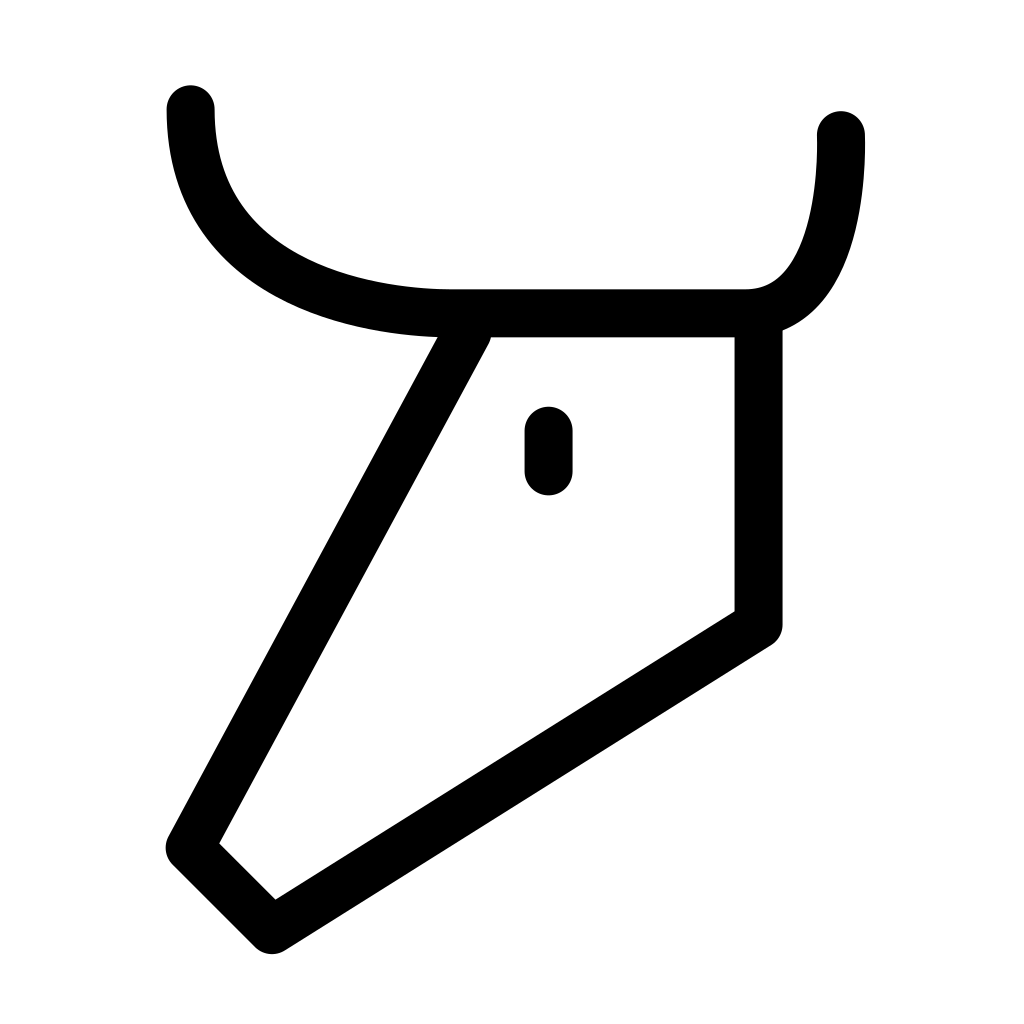
\includegraphics[scale=0.015]{pics/lection-14-ph-aleph-proto}
    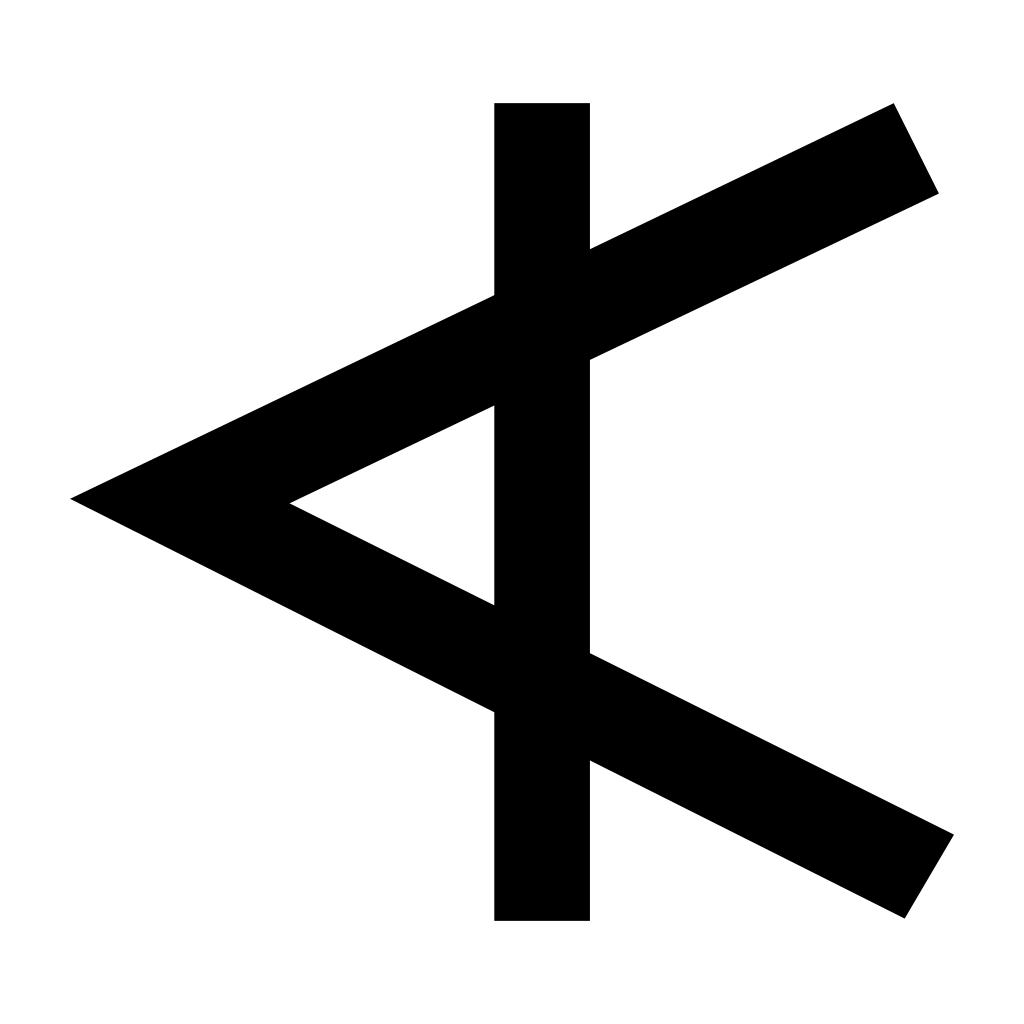
\includegraphics[scale=0.01]{pics/lection-14-ph-aleph}&  \Large $\alpha$, a, A, $\forall$  &  \Large $\aleph$\\
 голова быка &  'алп &  альфа &  алеф \\ &&& \\
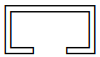
\includegraphics[scale=0.25]{pics/lection-14-house}
    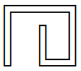
\includegraphics[scale=0.25]{pics/lection-14-courtyard} & 
    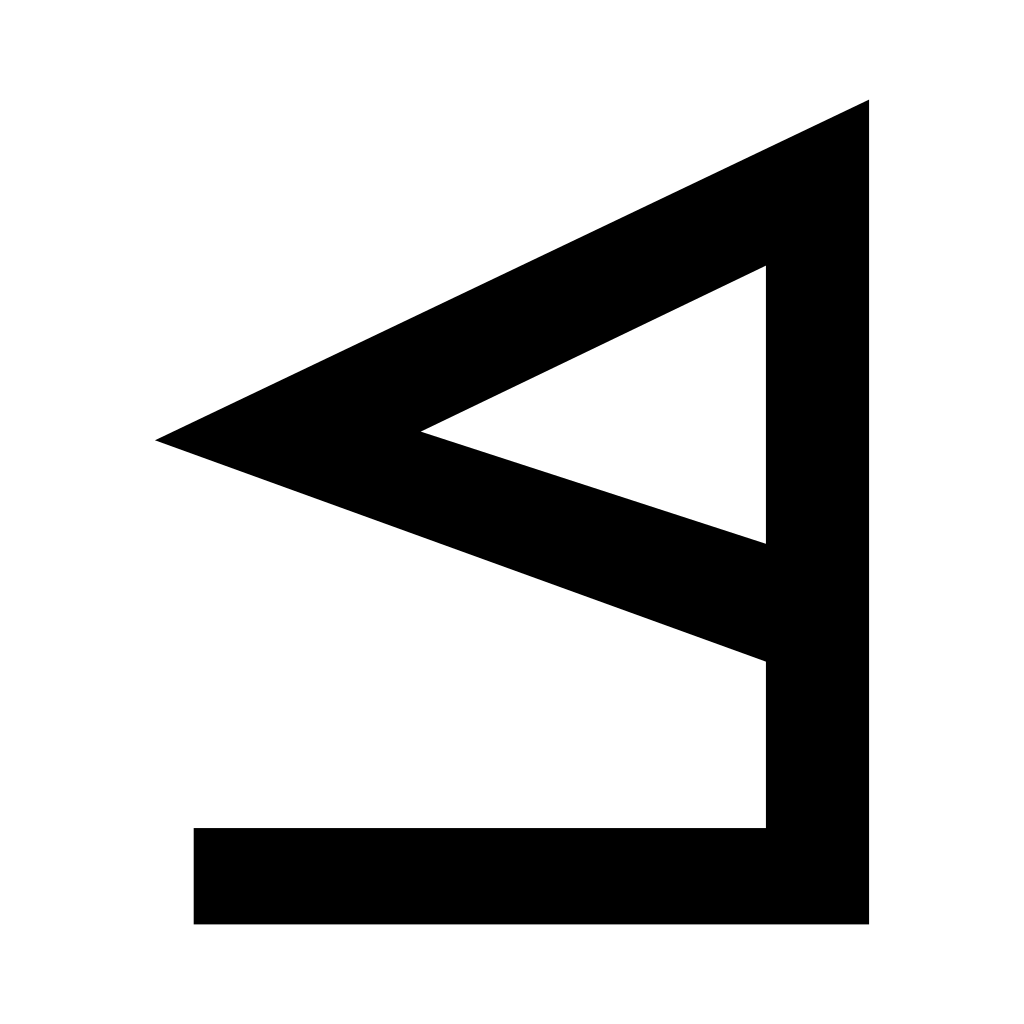
\includegraphics[scale=0.01]{pics/lection-14-ph-beth} & \Large $\beta$, B, Б & \Large $\beth$\\
дом/двор & бейт & бета & бет\\&&&\\

\includegraphics[scale=0.25]{pics/lection-14-throwstick} & 
    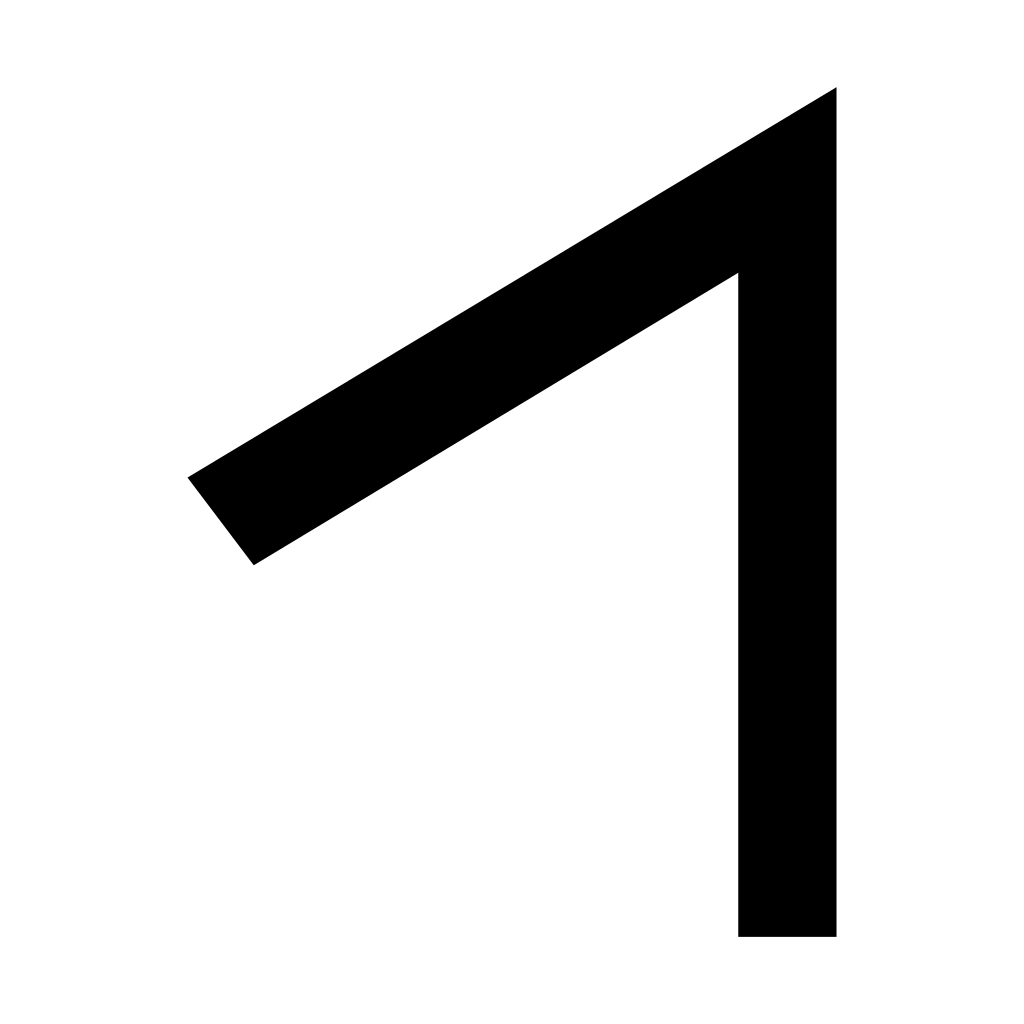
\includegraphics[scale=0.01]{pics/lection-14-ph-gimel} & \Large Г & \Large $\gimel$\\
 метательная палка & гамл & гамма & гимель\\&&&\\
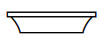
\includegraphics[scale=0.25]{pics/lection-14-door}
    
\includegraphics[scale=0.25]{pics/lection-14-fish} &
    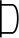
\includegraphics[scale=0.3]{pics/lection-14-ph-daleth-proto}
    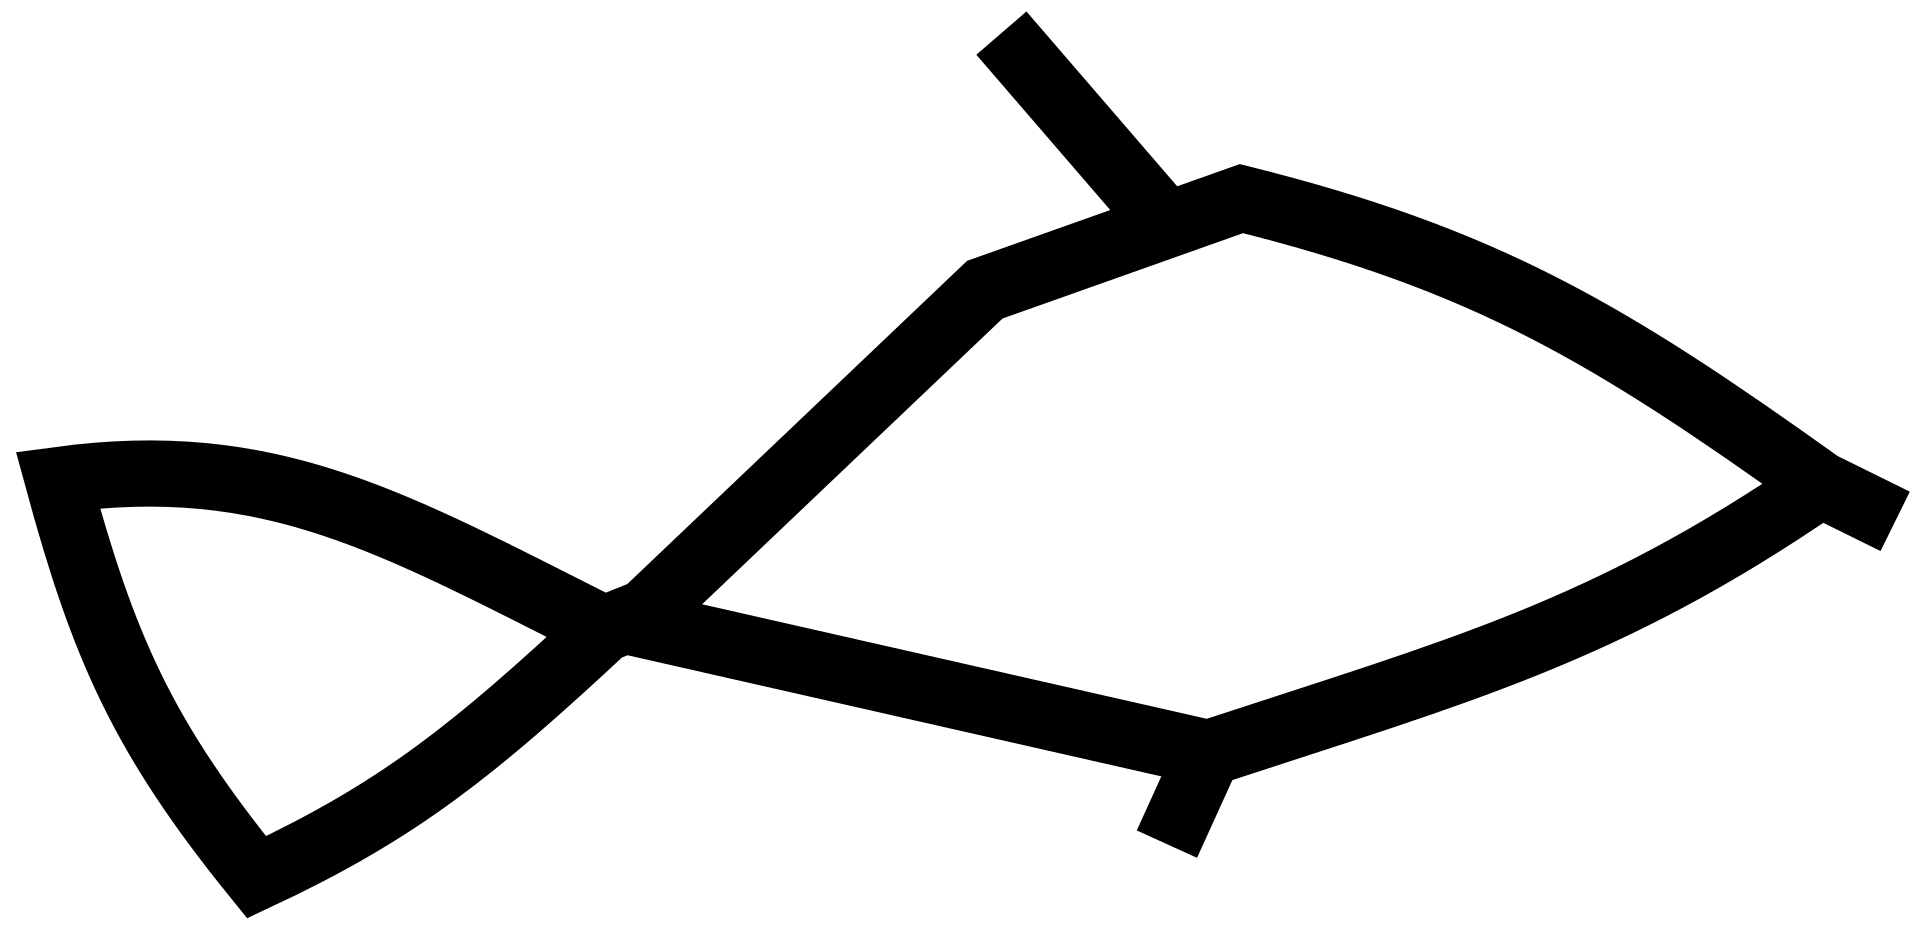
\includegraphics[scale=0.01]{pics/lection-14-ph-dag}
    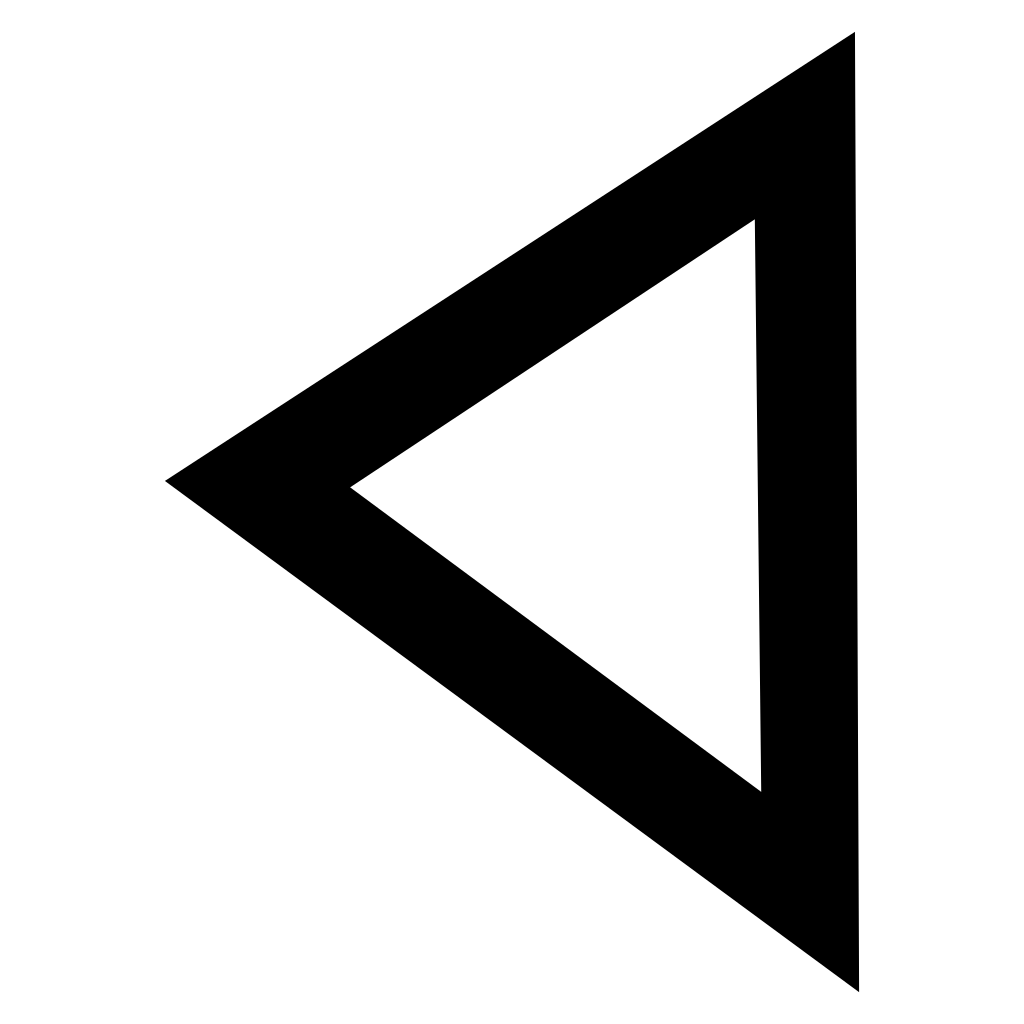
\includegraphics[scale=0.01]{pics/lection-14-ph-daleth} &  \Large $\Delta$, D, Д & 
    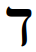
\includegraphics[scale=0.25]{pics/lection-14-daleth}\\
дверь/рыба & далт/даг & дельта & далет
\end{tabular}
\end{center}
\end{frame}

\begin{frame}{Иерархии $\aleph_n$ и $\beth_n$}
\begin{dfn}$\aleph_0 := |\omega|$; $\aleph_{k+1} := \min\{ a\ |\ a\text{ -- ординал},\aleph_k < |a|\}$\end{dfn}
\begin{dfn}$\beth_0 := |\omega|$; $\beth_{k+1} := |\mathcal{P}(\beth_k)|$\end{dfn}

Континуум-гипотеза (Г.Кантор, 1877): $\aleph_1 = \beth_1$ (не существует мощности, промежуточной 
между счётной и континуумом).

Обобщённая континуум-гипотеза: $\aleph_n = \beth_n$ при всех $n$.

\begin{dfn}Утверждение $\alpha$ противоречит аксиоматике: $\vdash\alpha$ ведёт к противоречию.

Утверждение $\alpha$ не зависит от аксиоматики: $\not\vdash\alpha$ и $\not\vdash\neg\alpha$.\end{dfn}\pause

\begin{thm}[О независимости континуум-гипотезы, Дж.Коэн, 1963] Утверждение $\aleph_1 = \beth_1$
не зависит от аксиоматики ZFC.\end{thm}
\end{frame}

\begin{frame}{Примеры мощностей множеств}
\begin{center}\begin{tabular}{l|l}Пример & мощность\\\hline
$\omega$ & $\aleph_0$\\
$\omega^2$, $\omega^\omega$ & $\aleph_0$\\
$\mathbb{R}$ & $\beth_1$\\
все непрерывные функции $\mathbb{R}\rightarrow\mathbb{R}$ & $\beth_1$\\
все функции $\mathbb{R}\rightarrow\mathbb{R}$ & $\beth_2$
\end{tabular}\end{center}

\end{frame}
%\newcommand{\divisible}%                                                     
%{\mathrel{\lower.2ex%
%\vbox{\baselineskip=0.7ex\lineskiplimit=0pt%
%\kern6pt \hbox{.}\hbox{.}\hbox{.}}%
%}}

%\begin{document}

%\newcommand\doubleplus{+\kern-1.3ex+\kern0.8ex}
%\newcommand\mdoubleplus{\ensuremath{\mathbin{+\mkern-10mu+}}}

%\begin{frame}{}
%\LARGE\begin{center}Теорема Лёвенгейма-Сколема\end{center}
%\end{frame}

\begin{frame}{Арифметика для кардинальных чисел}
\begin{dfn}Если $\alpha$ и $\beta$ --- кардинальные числа, то 
$\alpha + \beta := |\alpha\uplus\beta|$,
$\alpha \cdot \beta := |\alpha \times \beta|$, 
$\alpha ^\beta$ --- мощность множества всех функций из $\beta$ в $\alpha$\end{dfn}

\begin{thm}Если $\alpha$ --- некоторое бесконечное кардинальное число, то $\alpha\cdot\alpha = \alpha$\end{thm}

\begin{thm}Если $0 < \beta \le \alpha$ и $\alpha$ бесконечное, то $\alpha\cdot\beta = \alpha$\end{thm}
\begin{proof}
\begin{itemize}
\item $\alpha \cdot \beta \ge \alpha$:
фиксируем $b_0 \in \beta$ (т.к. $\beta > 0$), тогда
в качестве $f : \alpha \rightarrow \alpha \times \beta$ возьмём $f(a) = \langle a,b_0\rangle$.
\item $\alpha \cdot \beta \le \alpha \cdot \alpha = \alpha$.
\end{itemize}
\end{proof}\vspace{0.5cm}
\end{frame}

\begin{frame}{Как пересчитать вещественные числа (неформально)?}
\begin{enumerate}
\item Номер вещественного числа --- первое упоминание в литературе, т.е. $\langle j, y, n, p, r, c \rangle$:\\
j --- гёделев номер названия научного журнала (книги);\\
y --- год издания;\\
n --- номер;\\
p --- страница;\\
r --- строка;\\
c --- позиция\pause
\item Попробуете предъявить число $x$, не имеющее номера? Это рассуждение сразу даст номер.\\
\end{enumerate}
\end{frame}

\begin{frame}{Мощность модели и аксиоматизации}
\begin{dfn} Пусть задана модель $\langle D, F_n, P_n \rangle$ для некоторой теории первого порядка. 
Её мощностью будем считать мощность $D$.
\end{dfn}\pause

\begin{dfn} Пусть задана формальная теория с аксиомами $\alpha_n$. Её мощность --- мощность множества $\{\alpha_n\}$.
\end{dfn}\pause

\begin{exm} Формальная арифметика, исчисление предикатов, исчисление высказываний --- счётно-аксиоматизируемые.
\end{exm}
\end{frame}

\begin{frame}{Элементарная подмодель}
\begin{dfn}$\mathcal{M}' = \langle D', F'_n, P'_n \rangle$ --- элементарная подмодель $\mathcal{M} = \langle D, F_n, P_n \rangle$, 
если: \pause
\begin{enumerate}
\item $D' \subseteq D$, \pause $F'_n$, $P'_n$ --- сужение $F_n$, $P_n$ (замкнутое на $D'$). \pause
\item $\mathcal{M}\models \varphi(x_1,\dots,x_n)$ тогда и только тогда, когда $\mathcal{M}'\models \varphi(x_1,\dots,x_n)$
при $x_i \in D'$. \pause
\end{enumerate}
\end{dfn}

\begin{exm}Когда сужение $M$ не является элементарной подмоделью? \pause

$\forall x.\exists y.x \ne y$. Истинно в $\mathbb{N}$. \pause Но пусть $D' = \{ 0 \}$.
\end{exm}
\end{frame}

\begin{frame}{Теорема Лёвенгейма-Сколема}
\begin{thm}Пусть $T$ --- множество всех формул теории первого порядка. 
Пусть теория имеет некоторую модель $\mathcal{M}$.
Тогда найдётся элементарная подмодель $\mathcal{M'}$, причём $|\mathcal{M'}| \leq \max(\aleph_0, |T|)$.
\end{thm}\pause

\begin{proof} (Схема доказательства)
\begin{enumerate} 
\item Построим $D_0$ --- множество всех значений, которые упомянуты в языке теории. \pause
\item Будем последовательно пополнять $D_i$: $D_0 \subseteq D_1 \subseteq D_2 \dots$, следя за мощностью.
$D' = \cup D_i$.
\item Покажем, что $\langle D', F_n, P_n\rangle$ --- требуемая подмодель.
\end{enumerate}
\end{proof}
\end{frame}

\begin{frame}{Начальный $D_0$}
Пусть $\{f^0_k\}$ --- все 0-местные функциональные символы теории. \pause
\begin{enumerate}
\item $D_0 = \{ \llbracket f^0_k \rrbracket \}$, если есть хотя бы один $f^0_k$. \pause
\item Если таких $f^0_k$ нет, возьмём какое-нибудь одно значение из $D$. \pause
\end{enumerate}\pause

Очевидно, $|D_0| \le |T|$.
\end{frame}

\begin{frame}{Пополнение $D$}
Фиксируем некоторый $D_k$. Напомним, $T$ --- множество всех формул теории. Рассмотрим $\varphi \in T$.\pause
\begin{enumerate}
\item $\varphi$ не имеет свободных переменных --- пропустим. \pause
\item $\varphi$ имеет хотя бы одну свободную переменную $y$. \pause
\begin{enumerate}
\item $\varphi (y, x_1, \dots, x_n)$ при $y,x_i \in D_k$ бывает истинным и ложным --- ничего не меняем \pause
\item $\varphi (y, x_1, \dots, x_n)$ при $y \in D$ и $x_i \in D_k$ либо всегда истинен, либо всегда ложен --- ничего не меняем \pause
\item $\varphi (y, x_1, \dots, x_n)$ при $y,x_i \in D_k$ тождественно истинен или ложен, но при 
$y' \in D \setminus D_k$ отличается --- добавим $y'$ к $D_{k+1}$. \pause
Вместе добавим всевозможные $\llbracket\theta(y')\rrbracket$.
\end{enumerate}
\end{enumerate}\pause

\end{frame}

\begin{frame}{Оценка мощности $D'$}

\begin{enumerate}
\item Всего добавили не больше $|T| \cdot |T|$ (для каждой формулы $\varphi$, возможно, будет добавлен $y$ --- 
и всевозможные выражения $\theta(y)$, допустимые в языке), и $|D_0| \le |T| \le |T|\cdot|T|$,
отсюда $|D_k| \le |T| \cdot |T|$.
\item $|D'| = |\bigcup D_i| \le |T| \cdot |T| \cdot \aleph_0$.
\item Тогда $|T| \cdot |T| \cdot \aleph_0 = \max(|T|,\aleph_0)$. Разберём случаи:

\begin{enumerate}
\item Если $|T| < \aleph_0$, тогда $(|T| \cdot |T|) \cdot \aleph_0 = \aleph_0$
\item Если $|T| \ge \aleph_0$, тогда $(|T| \cdot |T|) \cdot \aleph_0 = |T| \cdot \aleph_0 = |T|$.

\end{enumerate}
\item Итого, $|D'| \le \max(|T|,\aleph_0)$.
\end{enumerate}

\end{frame}

\begin{frame}{$\mathcal{M}'$ --- элементарная подмодель}
Индукцией по структуре формул $\tau \in T$ покажем, 
что все формулы можно вычислить, и что $\llbracket \varphi \rrbracket_\mathcal{M'} = \llbracket \varphi \rrbracket_\mathcal{M}$.\pause

\begin{enumerate}
\item База, 0 связок. $\tau \equiv P(f_1(x_1,\dots,x_n),\dots,f_n(x_1,\dots,x_n))$. \pause Если $x_i \in D'$, то значит,
добавлены на некоторых шагах (максимальный пусть $t$). Поэтому в $D_{t+1}$ можно вычислить формулу, и её значение сохранилось. \pause
\item Переход. Пусть формулы из $k$ связок сохраняют значения. Рассмотрим $\tau$ с $k+1$ связкой. \pause
\begin{enumerate}
\item $\tau \equiv \rho \star \sigma$ --- очевидно. \pause
\item $\tau\equiv\forall y.\varphi(y,x_1,\dots,x_n)$. \pause 
Каждый $x_i$ добавлен на каком-то шаге --- максимум $t$. \pause 
Если $\varphi(y,x_1,\dots,x_n)$ бывает истинен и ложен при $y_t, y_f \in D$, то $y_t, y_f \in D_{t+1}$ (по построению). \pause
Поэтому, если $\mathcal{M}\not\models\forall y.\varphi(y,x_1,\dots,x_n)$, то и 
$\mathcal{M'}\not\models\forall y.\varphi(y,x_1,\dots,x_n)$. \pause
Если же $\varphi(y,x_1,\dots,x_n)$ не меняется от $y$, то тем более
$\llbracket \varphi \rrbracket_\mathcal{M'} = \llbracket \varphi \rrbracket_\mathcal{M}$. \pause
\item $\tau\equiv\exists y.\varphi(y,x_1,\dots,x_n)$ --- аналогично.
\end{enumerate}
\end{enumerate}
\end{frame}

\begin{frame}{<<Парадокс>> Сколема}
\begin{enumerate}
\item Как известно, $|\mathbb{R}| = |\mathcal{P}(\mathbb{N})| > |\mathbb{N}| = \aleph_0$. \pause Однако, ZFC --- теория со счётным
количеством формул. \pause
Значит, существует счётная модель ZFC, то есть $|\mathbb{R}| = \aleph_0$. \pause В чём ошибка? \pause
\item У равенств разный смысл, первое --- в предметном языке, второе --- в метаязыке. 
\end{enumerate}
\end{frame}

\end{document}
